% Institute of Computer Science thesis template
% authors: Sven Laur, Liina Kamm
% last change Tõnu Tamme 09.05.2017
%--
% Compilation instructions:
% 1. Choose main language on line 55-56 (English or Estonian)
% 2. Compile 1-3 times to get refences right
% pdflatex bachelors-thesis-template
% bibtex bachelors-thesis-template
%--
% Please use references like this:
% <text> <non-breaking-space> <cite/ref-command> <punctuation>
% This is an example~\cite{example}.

\documentclass[12pt]{article}

% A package for setting layout and margins for your thesis 
\usepackage[a4paper]{geometry}

%%=== A4 page setup ===
%\setlength{\paperwidth}{21.0cm} 
%\setlength{\paperheight}{29.7cm}
%\setlength{\textwidth}{16cm}
%\setlength{\textheight}{25cm}


% When you write in Estonian then you want to use text with right character set
% By default LaTeX does not know what to do with õäöu letters. You have to specify
% a correct input and font encoding. For that you have to Google the Web     
%
% For TexShop under MacOS X. The right lines are 
%\usepackage[applemac]{inputenc}
%\usepackage[T1]{fontenc} %Absolutely critical for *hyphenation* of words with non-ASCII letters.
%
% For Windows and Linux the right magic lines are   
% \usepackage[latin1]{inputenc}
% \usepackage[latin5]{inputenc}
%%\usepackage[utf8]{inputenc} %Package inputenc Error: Unicode char ´ (U+B4) not set up for use with LaTeX
\usepackage[utf8x]{inputenc}
\usepackage[T1]{fontenc} %Absolutely critical for *hyphenation* of words with non-ASCII letters.

% Typeset text in Times Roman instead of Computer Modern (EC)
\usepackage{times}

% Suggested packages:
\usepackage{microtype}  %towards typographic perfection...
\usepackage{inconsolata} %nicer font for code listings. (Use \ttfamily for lstinline bastype)


% Use package babel for English or Estonian 
% If you use Estonian make sure that Estonian hyphenation is installed 
% - hypen-estonian or eehyp packages
%
%===Choose the main language in thesis
\usepackage[estonian, english]{babel} %the thesis is in English 
%\usepackage[english, estonian]{babel} %the thesis is in Estonian


% Change Babel document elements 
\addto\captionsestonian{%
  \renewcommand{\refname}{Viidatud kirjandus}%
  \renewcommand{\appendixname}{Lisad}%
}


% If you have problems with Estonian keywords in the bibliography
%\usepackage{biblatex}
%\usepackage[backend=biber]{biblatex}
%\usepackage[style=alphabetic]{biblatex}
% plain --> \usepackage[style=numeric]{biblatex}
% abbrv --> \usepackage[style=numeric,firstinits=true]{biblatex}
% unsrt --> \usepackage[style=numeric,sorting=none]{biblatex}
% alpha --> \usepackage[style=alphabetic]{biblatex}
%\DefineBibliographyStrings{estonian}{and={ja}}
%\addbibresource{bachelor-thesis.bib}



% General packages for math in general, theorems and symbols 
% Read ftp://ftp.ams.org/ams/doc/amsmath/short-math-guide.pdf for further information
\usepackage{amsmath} 
\usepackage{amsthm}
\usepackage{amssymb}

% Optional calligraphic fonts    
% \usepackage[mathscr]{eucal}

% Print a dot instead of colon in table or figure captions
\usepackage[labelsep=period]{caption}

% Packages for building tables and tabulars 
\usepackage{array}
\usepackage{tabu}   % Wide lines in tables
\usepackage{xspace} % Non-eatable spaces in macros
\usepackage{booktabs}
\usepackage{longtable}

% Including graphical images and setting the figure directory
\usepackage{graphicx}
\graphicspath{{figures/}}

% Packages for getting clickable links in PDF file
%\usepackage{hyperref}
\usepackage[hidelinks]{hyperref} %hide red (blue,green) boxes around links
\usepackage[all]{hypcap}


% Packages for defining colourful text together with some colours
\usepackage{color}
\usepackage{xcolor} 
%\definecolor{dkgreen}{rgb}{0,0.6,0}
%\definecolor{gray}{rgb}{0.5,0.5,0.5}
\definecolor{mauve}{rgb}{0.58,0,0.82}


% Standard package for drawing algorithms
% Since the thesis in article format we must define \chapter for
% the package algorithm2e (otherwise obscure errors occur) 
\let\chapter\section
\usepackage[ruled, vlined, linesnumbered]{algorithm2e}

% Fix a  set of keywords which you use inside algorithms
\SetKw{True}{true}
\SetKw{False}{false}
\SetKwData{typeInt}{Int}
\SetKwData{typeRat}{Rat}
\SetKwData{Defined}{Defined}
\SetKwFunction{parseStatement}{parseStatement}


% Nice todo notes
\usepackage{todonotes}

% comments and verbatim text (code)
\usepackage{verbatim}


% Proper way to create coloured code listings
\usepackage{listings}
\lstset{ 
  %language=python,                % the language of the code
  language=C++,
  basicstyle=\footnotesize,        % the size of the fonts that are used for the code
  %numbers=left,                   % where to put the line-numbers
  %numberstyle=\footnotesize,      % the size of the fonts that are used for the line-numbers
  numberstyle=\tiny\color{gray}, 
  stepnumber=1,                    % the step between two line-numbers. If it's 1, each line 
                                   % will be numbered
  numbersep=5pt,                   % how far the line-numbers are from the code
  backgroundcolor=\color{white},   % choose the background color. You must add \usepackage{color}
  showspaces=false,                % show spaces adding particular underscores
  showstringspaces=false,          % underline spaces within strings
  showtabs=false,                  % show tabs within strings adding particular underscores
  frame = lines,
  %frame=single,                   % adds a frame around the code
  rulecolor=\color{black},		   % if not set, the frame-color may be changed on line-breaks within 
                                   % not-black text (e.g. commens (green here))
  tabsize=2,                       % sets default tabsize to 2 spaces
  captionpos=b,                    % sets the caption-position to bottom
  breaklines=true,                 % sets automatic line breaking
  breakatwhitespace=false,         % sets if automatic breaks should only happen at whitespace
  %title=\lstname,                 % show the filename of files included with \lstinputlisting;
                                   % also try caption instead of title
  keywordstyle=\color{blue},       % keyword style
  commentstyle=\color{dkgreen},    % comment style
  stringstyle=\color{mauve},       % string literal style
  escapeinside={\%*}{*)},          % if you want to add a comment within your code
  morekeywords={*,game, fun}       % if you want to add more keywords to the set
}


% Obscure packages to write logic formulae and program semantics
% Unless you do a bachelor thesis on program semantics or static code analysis you do not need that
% http://logicmatters.net/resources/ndexamples/proofsty3.html <= writing type rules => use semantic::inference
% ftp://tug.ctan.org/tex-archive/macros/latex/contrib/semantic/semantic.pdf
\usepackage{proof}
\usepackage{semantic} 
\setlength{\inferLineSkip}{4pt}
\def\predicatebegin #1\predicateend{$\Gamma \vdash #1$}

% If you really want to draw figures in LaTeX use packages tikz or pstricks
% However, getting a corresponding illustrations is really painful  


% Define your favorite macros that you use inside the thesis 
% Name followed by non-removable space
\newcommand{\proveit}{ProveIt\xspace}

% Macros that make sure that the math mode is set
\newcommand{\typeF}[1] {\ensuremath{\mathsf{type_{#1}}}\xspace}
\newcommand{\opDiv}{\ensuremath{\backslash \mathsf{div}}\xspace} 

% Nice Todo box
\newcommand{\TODO}{\todo[inline]}

% A way to define theorems and lemmata
\newtheorem{theorem}{Theorem}



%%% BEGIN DOCUMENT
\begin{document}

%===BEGIN TITLE PAGE
\thispagestyle{empty}
\begin{center}

\iflanguage{english}{%
\large
UNIVERSITY OF TARTU\\%[2mm]
Institute of Computer Science\\
Computer Science Curriculum\\%[2mm]
}{%
TARTU ÜLIKOOL\\
Arvutiteaduse instituut\\
Informaatika õppekava\\%[2mm]
}%\iflanguage

%\vspace*{\stretch{5}}
\vspace{25mm}

\Large Yevhen Tyshchenko

\vspace{4mm}

\huge Thesis Title

%\vspace*{\stretch{7}}
\vspace{20mm}

\iflanguage{english}{%
\Large Master's Thesis (30 ECTS)
}{%
\Large Bakalaureusetöö (9 EAP)
}%\iflanguage

\end{center}

\vspace{2mm}

\begin{flushright}
 {
 \setlength{\extrarowheight}{5pt}
 \begin{tabular}{r l} 
  \sffamily \iflanguage{english}{Supervisor}{Juhendaja}: & \sffamily Kairit Sirts, PhD \\
 \end{tabular}
 }
\end{flushright}

%\vspace*{\stretch{3}}
%\vspace{10mm}

\vfill
\centerline{Tartu 2018}

%===END TITLE PAGE

% If the thesis is printed on both sides of the page then 
% the second page must be must be empty. Comment this out
% if you print only to one side of the page comment this out
%\newpage
%\thispagestyle{empty}    
%\phantom{Text to fill the page}
% END OF EXTRA PAGE WITHOUT NUMBER


%===COMPULSORY INFO PAGE
\newpage

%=== Info in English
\newcommand\EngInfo{{%
\selectlanguage{english}
\noindent\textbf{\large Type Inference for Fourth Order Logic Formulae}

\vspace*{3ex}

\noindent\textbf{Abstract:}

\noindent
\TODO{Abstract}
\vspace*{1ex}

\noindent\textbf{Keywords:}\\
\TODO{List of keywords}
%Layout, formatting, template

\vspace*{1ex}

\noindent\textbf{CERCS:}\TODO{CERCS code and name:~\url{https://www.etis.ee/Portal/Classifiers/Details/d3717f7b-bec8-4cd9-8ea4-c89cd56ca46e}}

\vspace*{1ex}
}}%\newcommand\EngInfo


%=== Info in Estonian
\newcommand\EstInfo{{%
\selectlanguage{estonian}
\noindent\textbf{\large Tüübituletus neljandat järku loogikavalemitele}
\vspace*{1ex}

\noindent\textbf{Lühikokkuvõte:} 

%\noindent ...

\TODO{One or two sentences providing a basic introduction to the field, comprehensible to a scientist in
any discipline.}
\TODO{Two to three sentences of
more detailed background, comprehensible to scientists in related disciplines.}
\TODO{One sentence clearly stating the general problem being addressed by this particular
study.}
\TODO{One sentence summarising the main result (with the words ``here we show´´ or their equivalent).}
\TODO{Two or three sentences explaining what
the main result reveals in direct
comparison to what was thought to be the case previously, or how the main result adds to previous knowledge.}
\TODO{One or two sentences to put the results into a more general context.}
\TODO{Two or three sentences to provide a
broader perspective, readily
comprehensible to a scientist in any
discipline, may be included in the first paragraph
if the editor considers that the accessibility of
the paper is significantly enhanced by their inclusion.}

\vspace*{1ex}

\noindent\textbf{Võtmesõnad:}\\
\TODO{List of keywords}
%Layout, formatting, template

\vspace*{1ex}

\noindent\textbf{CERCS:}\TODO{CERCS kood ja nimetus:~\url{https://www.etis.ee/Portal/Classifiers/Details/d3717f7b-bec8-4cd9-8ea4-c89cd56ca46e}}

\vspace*{1ex}
}}%\newcommand\EstInfo


%=== Determine the order of languages on Info page
\iflanguage{english}{\EngInfo}{\EstInfo}
\iflanguage{estonian}{\EngInfo}{\EstInfo}


\newpage
\tableofcontents


% Remember to remove this from the final thesis version
\newpage
\listoftodos[Unsolved issues]
% END OF TODO PAGE 


\newpage
\section{Introduction}
\TODO{What is it in simple terms (title)?}
\TODO{Why should anyone care?}
\TODO{What was my contribution?} 
\TODO{What you are doing in each section (a sentence or two per section)}
Usually the data about person's mental state is confidential and only doctors have an access for it. Fortunately, people tend to share their thoughts, stories and quite personal feelings on the web resources such as social network insights, blog platforms, forums etc. In particular, some research are based on Twitter posts data while others collect post entries from mental health support forums that are then labeled by metal health specialists. These resources are publicly available and often can be quired and filtered using keywords.

\newpage
\section{Previous Work} 
\TODO{Describe previous work}


\section{Technical background}
This section incorporates technical description of methods and approaches applied for this natural language processing task including web data retrieval, numerical text representation, probabilistic topic modeling, and text classification methods. In particular, web data extraction approaches are described in 3.1, text representation methods are covered in 3.2...
\subsection{Web data retrieval}
\TODO{Web data extraction, applications and techniques: A survey}
\TODO{A Brief Survey of Web Data Extraction Tools}

Web data information retrieval field has developed considerably since the rapid growth of Word Wide Web pages and websites. The existing approaches could be grouped into two categories by their underlying work principle: \textit{tree-based approaches}, \textit																																{web wrappers}.

The first category is \textit{tree-based approaches} that consider the DOM web page representation which is basically a labeled rooted tree hierarchy over a mixture of text and HTML tags. This particular web page representation motivates the usage of tree-based algorithms and mechanisms of addressing specific page tree nodes containing desired data. This is usually performed by XPath queries to a single page element or a group of similar page elements enclosed between HTML tags. 

The second category is \textit{web wrappers} that in terms of web data extraction is often described as a process aimed to find, extract, and transform an unstructured target data for further analysis by computer program in automated or semi-automated way. This approach could be decomposed on the following three steps:
\begin{enumerate}
	\item Initialization --- wrapper is created;
	\item Execution --- wrapper runs and collects the data;
	\item Maintenance --- if the data source structure changes then the respective wrapper should be also tuned to handle it.
\end{enumerate}

\subsection{Text representation}
\subsubsection{Bag-of-words}
Most of the natural language processing tasks require input text numerical representation rather than raw words meaning that each word must be encoded in order to be processed by machines. One of the most popular and straightforward approaches to encode text is to use a bag-of-words (BoW) text representation. This model encodes words with their frequencies and outputs a matrix where rows are documents and columns represent unique words. The word importance in this model is just its frequency which is the main weakness of this representation. In other words, frequently used words such as "the" that are not discriminative across the collection of the documents will get higher weights thus hiding the less frequent but more informative key words.
\subsubsection{Term Frequency-Inverse Document Frequency}
//////////////////////////////////////////////////
\TODO{Original paper G. Salton and M. McGill, editors. Introduction to Modern Information Retrieval. McGraw-Hill,	1983.}

Therefore, term frequency-inverse document frequency (TFIDF) is applied to resolve this issue. TFIDF is basically a numeric statistic that describes the importance of a word with respect to each document in a corpora. The term frequency (TF) cab be calculated as follows:

\begin{align*}
	tf(w, d)=\frac{n_w}{\sum_{k}^{}n_k},
\end{align*}
where $n_w$ is the number of times the word appeared in a document $d$ and $\sum_{k}^{}n_k$ is the total number of words in a document.

The inverse document frequency (IDF) diminishes the weights of frequent words and strengthen rare words if they don't appear often in other documents except the current one, and can be calculated as follows:
\begin{align*}
	idf(w, C)=log\frac{|C|}{|\{c\in{C}:w\in{c}\}|},
\end{align*} 
where $|C|$ is the corpus size and $|\{c\in{C}:t\in{c}\}|$ is the number of documents where the word $w$ appears. Finally, TFIDF itself is a product of the two aforementioned frequencies: 
\begin{align*}
	tfidf(w, d, C)=tf(w, d)\cdot{idf(w, C)}.
\end{align*}
The word will be ranked with greater TFIDF value if it is present in a particular document and absent in other documents.

\subsubsection{}


\subsection{Topic modeling}
Nowadays, the amounts of written text information often do not fit the computational capacity and make scientists apply text mining methods to discover useful hidden text structures or similarities. One important task in natural language processing field is detecting the between document similarities by ideas and topics mentioned there. Topic modeling is an unsupervised text mining approach that discovers these similarities in a text or corpora. Topic model itself refer to statistical algorithms that explore the topics over the collection of documents and helps to annotate these documents according to detected topics. 


\subsubsection{Latent Dirichlet Allocation}
//////////////////////////////////////////////////
\TODO{Original LDA paper http://www.jmlr.org/papers/volume3/blei03a/blei03a.pdf}

Latent Dirichlet Allocation (LDA) is a generative probabilistic model that models a text corpus and is helpful in discovering its underlying topic structures. The main idea behind LDA is that each document is represented as a probability distribution over latent topics. Every topic in this model is treated as a distribution over words existing in the collection of documents. The LDA model could be decomposed into two steps: \textit{model generation} and \textit{model inference}. 

\paragraph{Model generation:}
On model generation stage document-to-topic and topic-to-word distributions are drawn from two Dirichlet distributions with $\alpha$ and $\beta$ parameters. Then, for each word position in document choose topic and, finally, given the topic distribution pick the word for this position. LDA model is often represented using plate diagram (Figure \ref{fig:LDA_plate_notation}) with the following notations:
\begin{figure} [htbp]
	\centering
	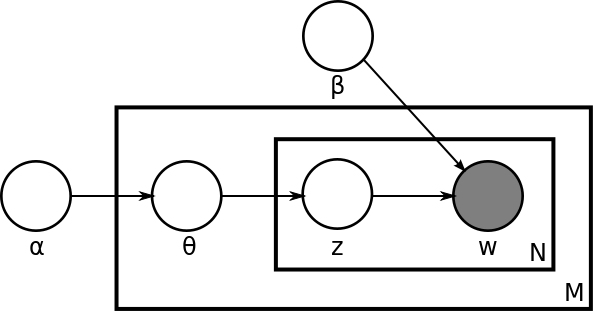
\includegraphics[width=0.5\textwidth]{LDA_plate}
	\caption{Plate notation of the LDA model.}
	\label{fig:LDA_plate_notation}
\end{figure}
\begin{itemize}
	\item {The number of topics $K$ is fixed and defined}.
	\item {The number of all documents in a corpus $D$ is $M$}.
	\item {$\phi_k$ is a $k$-th topic word distribution over a fixed vocabulary where ${1\leq k\leq K}$}.
	\item {$\Theta_m$ is a $m$-th document topic distribution where $1\leq m \leq M$}.
	\item {$z_m$ is the topic assignment for $m$-th document, and $z_{m,n}$ is the topic assignment for $n$-th word in $m$-th document}.
	\item {$w_{m, n}$ is actually the $n$-th word in $m$-th document}.
	\item {$\alpha, \beta$ are hyperparameters of a Dirichlet distribution.}
\end{itemize}
Then, the generative process could be described in following steps:
\begin{enumerate}
	\item $\forall$ document $d_i\in D$ draw $\Theta_{d_i} \sim Dirichlet(\alpha)$ 
	\item $\forall$ topic $k \in K$ draw $\phi_k \sim Dirichlet(\beta)$
	\item $\forall \,i,\,j\!: 1\leq i \leq M, 1 \leq j \leq |d_i|$ where $|d_i|$ is the number of selected words in document $d_i$ draw:
	\begin{itemize}
		\item {topic $z_{i,j}\sim Multinomial(\Theta_i)$}
		\item {word $w_{i,j}\sim Multinomial(\phi_{z_{i,j}})$}
	\end{itemize}
\end{enumerate}

\paragraph{Model inference:}
Now the task is to infer word-to-topic assignments $z_{i,j}$, document-to-topic distributions $\Theta_i$ and corpus topic distributions $\phi_k$. The original paper [Blei] suggests a \textit{variational inference} approach to estimate the posterior distribution of the hidden variable $w$ --- gray circle on figure \ref{fig:LDA_plate_notation}. 


\TODO{describe batch variational Bayes: Online Learning for Latent Dirichlet Allocation article}
\TODO{add formulas $https://www.cl.cam.ac.uk/teaching/1213/L101/clark_lectures/lect7.pdf$}
\TODO{http://www.ece.umd.edu/~smiran/LDA.pdf}

Finally, apart from the vector space corpus representation LDA outputs document-to-topic and word-to-topic distribution matrices which are useful for further topic analysis, and, for instance, can be applied as features for text classification tasks.

\subsection{Classification}
\subsubsection{Support Vector Machines}
//////////////////////////////////////////////////
\TODO{Original paper https://rdcu.be/MlPW}
Support Vector Machine (SVM) is a supervised machine learning method that can be used for both classification and regression tasks. The main idea behind it is to divide a linearly separable data into two classes with maximum between-class distance. If we consider two-dimensional example illustrated on Figure? SVM finds an optimal line or set of lines that lie as far from the nearest class data points as possible. The dashed lines are called support vectors.
\begin{figure} [htbp]
	\centering
	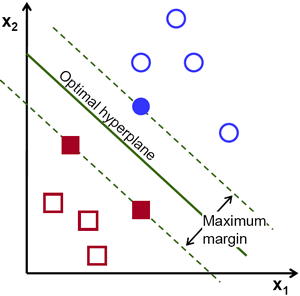
\includegraphics[width=0.5\textwidth]{svm_illustration}
	\caption{SVM illustration for two-dimensional case.}
	\label{fig:svm_illustartion}
\end{figure}
\TODO{link to image: https://www.quora.com/What-does-support-vector-machine-SVM-mean-in-laymans-terms}
In general, SVM finds an optimal hyperplane or a set of hyperplanes in high-dimensional space that separate the input data with the maximum margin between this hyperplane and nearest training data points of any class. If the input data is not linearly separable a kernel function is applied to map it into higher-dimensional space to make it linearly separable. The most popular non-linear kernels are: polynomial kernel, Gaussian radial basis function, and sigmoid kernel. 

\subsubsection{Convolutional Neural Networks}
//////////////////////////////////////////////////
\TODO{what is CNN?}
\TODO{CNN architecture}
\TODO{CNN layers}


\clearpage %if newpage doesn't work
\section{Method} 
\subsection{Data scraping} 
\TODO{Scraping procedure flowchart}
Web data retrieval technique applied in this work falls into the category of web wrappers although the XPath queries were used to get specific DOM elements. The goal of this step is to extract two corpus of blog posts: control and clinical, such that they will be similar in terms of the discussed topics.

The data for this work was extracted from the Blogger platform in an semi-automated way using Python script and Selenium package for browser automation. Initially, the idea was to collect the control and clinical blogs by keyword interest "\textit{depression}" using the platform built-in filter, then manually verify scraped blog URLs, and finally get desired blog posts by these URLs using scrapper. The drawback of the built-in filter is that it brought mostly control group containing psychiatrists, volunteers, psychologists and blogs about religion. Therefore, another query was constructed with the help of Google Advanced Search tool and can be interpreted as follows: 
\begin{itemize}
	\item Find pages such that contain all these words: \textit{my, life, clinical, depression, anxiety}
	\item Any of the words: \textit{anxiety, depression}
	\item Within the website: \textit{blogspot.com}.
\end{itemize}
\begin{align*}
	\textit{my life clinical depression anxiety  anxiety OR depression OR disorder site:blogspot.com}
\end{align*}
 This detailed search query brought much more blogs where people mention their clinical or self-stated diagnosis.

 The scraping method introduced more than 100 blog links that were then manually evaluated. This brought in 47 clinical and 36 control subject blogs which were then scraped entirely. All in all, there are 10799 and 6176 control and clinical blog posts respectively, and later restricted to the same size to avoid data imbalance.
 
\subsection{Data preprocessing}
\TODO{Yoon Kim paper $https://arxiv.org/pdf/1408.5882.pdf$}
\TODO{Yoon Kim code $https://github.com/yoonkim/$}
This section describes data preprocessing - a vital step in any natural language processing task. Firstly, all input data was cleaned using regular expressions which are actually the sequences of characters that define the search string in a text. In particular, the initial string cleaning pipeline were taken from the Yoon Kim's preprocessing code, modified and extended with additional regular expressions matching and replacing the URL addresses, contractions and redundant whitespaces with a single whitespace. Additionally, brackets, colons, dashes, punctuation marks, contractions and all newline symbols were removed. Finally, the posts were lowercased and saved as separate text files in order to perform the preprocessing step only once thus considerably reducing the overall execution time.

In order to prevent an undesirable impact on final topic model the most frequent and rare words were removed. In particular, the word was filtered out if it occurs in less than $3$ documents or more than $80\%$ of all documents. However, further experiments on non-filtered data showed better classification results so this cleaning step was rejected.

The \textit{lemmatization} were chosen because unlike \textit{stemming} it aims to remove word endings based on vocabulary and morphological word analysis. This ensures that the word endings will not be roughly dropped often resulting in senseless word pieces (\textit{stemming}) but rather transformed into word lemmas conformant with dictionary. For example, the lemmatization output for words \textit{"good", "better", "best"} is just the common lemma \textit{"good"} while stemming will result in \textit{"good", "bet", "best"}. Furthermore, all words were enriched with \textit{part-of-speech tags} (POS-tags) to represent their word classes and improve lemmatization results.

Then, the data was split into three parts statically with 70\%, 15\% and 15\% partitions sizes for training, development and test set respectively. To ensure that each author belongs to only one partition splitting was done based on blog sizes measured in number of posts per author. Moreover, it was attempted to keep the distribution of blog sizes similar across these parts so as to prevent data imbalance.

The bag of words text representation was constructed using the scikit-learn CountVectorizer with $100000$ features i.e. word tokens. It produced a sparse matrix representation of a corpus $n \times m$ where $n$ stands for the number of documents in corpus and $m$ is the number of features.


\subsection{Topic modeling}
\label{method_topic_modelling}
//////////////////////////////////////////////////
\TODO{Topic modelling and methods 
	http://www.cs.columbia.edu/~blei/papers/BleiLafferty2009.pdf}
Topic modeling experiments were performed using the \textit{scikit-learn} Python LDA implementation. Out-of-the-box method also allows to choose the learning method for the model either \textit{"online"} or \textit{"batch"}. The main difference between these methods is that \textit{"online"} parameter refers to Online variational Bayes method which uses a mini-batch of data on each iteration to update the resulting document-to-topic matrix while \textit{"batch"} refers to Batch variational Bayes method and uses all data to update this matrix on each step. The latter method was chosen because the final model will be trained only once and the amount of input data is fixed and small enough to treat it as a single batch. 

\TODO {Papers with topic model evaluation approaches.}
\subsubsection{Model evaluation and parameter search}
\label{eval_param_search}
The optimal number of $n$ topics for the model was chosen based on the classification performance of previously tuned SVM classifier using the grid search parameter optimization procedure. 


\subsection{Classification setup}
\TODO{What methods will be covered?}
\TODO{Why they were used?}
This section provides the optimal configurations applied for the classification methods and describes their technical details. Additionally, it also discusses the evaluation measures used in this work.
\paragraph{LDA+SVM}
The initial approach is similar to [Blei] and consists of SVM classifier on top of LDA features. SVM implementation was taken from the \textit{scikit-learn} library. The optimal SVM parameters were tuned with the built-in parameter search procedure and fixed: regularization term $C=xx$ and $gamma=yy$. 

\section{Results and analysis}
This section covers the topic modeling results in section \ref{topic_modeling_results}, and provides the performance tables for the applied classification methods 6.2. 

\subsection{Topic model}
\label{topic_modeling_results}
The resulting LDA model requires further analysis to reach better understanding of the scraped data. The topic model parameter search procedure described in \ref{eval_param_search} resulted in the best classification score of $blabla$ with $blaaa$ topics. It was also observed that SVM's accuracy fluctuated during the parameter tuning as illustrated on Figure $100500 top figure$.
\TODO{topic number vs svm accuracy plot}
Particularly, the highest classification accuracies were faced with $n$ and $m$ topic numbers that unexpectedly differ quite a lot. Thus, the topics were manually investigated and labeled according to their twenty most representative words. 
To evaluate the scraped data in terms of its topic model two document-to-topic probability distribution matrices for control and clinical text corpus were visualized on \ref{fig:doc2topic_heatmaps}. They outlined the shift towards $some topic$ in clinical group comparing to controls. Potentially, this imbalance could make classifier predict based on topic assignments so the aim was to statistically estimate how dependent are these two categorical variables: \textit{control} and \textit{clinical}. 
\TODO{The Chi-square test of independence Mary L. McHugh}
This work covers the results of two statistical tests: \textit{Chi-square test of independence} and \textit{Fisher's exact test}. They both require a contingency table as input so the one was constructed with 15 columns (LDA topics) and two rows --- \textit{control} and \textit{clinical} that contain document counts (Figure $100$).



\begin{figure} [htbp]
	\begin{tabular}{c c}
		%
		\begin{minipage}{0.47\textwidth}
			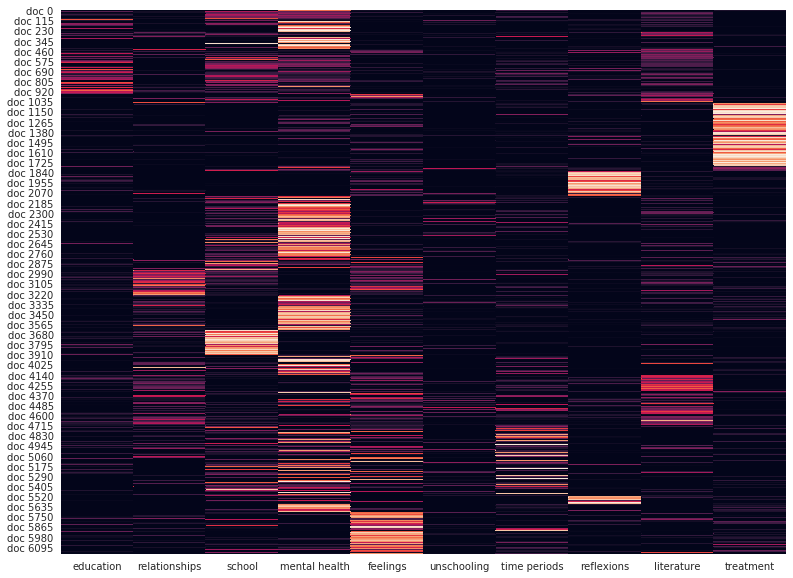
\includegraphics[width=\textwidth]{control_doc2topic}
		\end{minipage}
		%
		&
		\begin{minipage}{0.50\textwidth}
			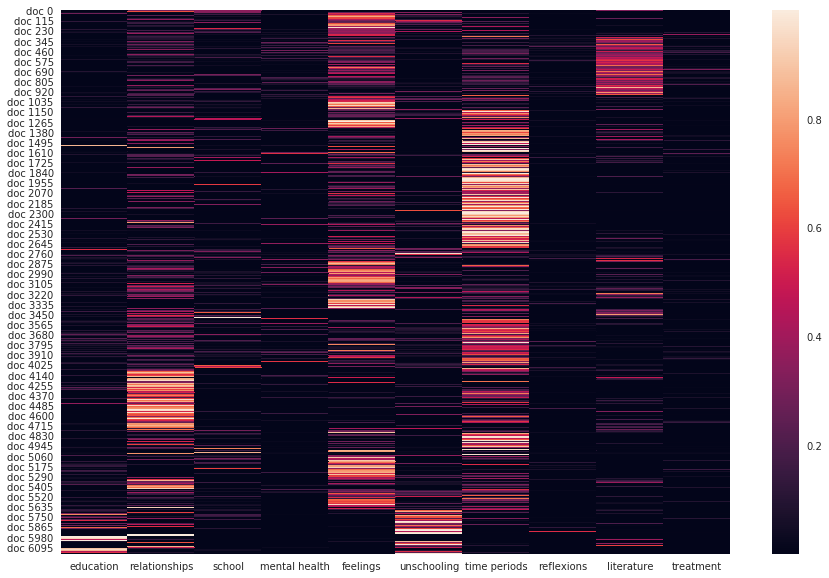
\includegraphics[width=\textwidth]{clinical_doc2topic}
		\end{minipage}
	\end{tabular}
	%
	\caption{Heatmap visualizations of document-to-topic probabilities for control (\textit{left}) and clinical (\textit{right}) text corpuses. }
	\label{fig:doc2topic_heatmaps}
\end{figure}

The resulting document-to-topic distribution analysis showed that the assumptions about the data collection were confirmed.  

\begin{longtable}[c]{|l|l|}
	\caption{My caption}
	\label{my-label}\\
	\hline
	\multicolumn{1}{|c|}{} & \begin{tabular}[c]{@{}l@{}}school student counselor college high resource peer \\ counseling program teen parent teacher information \\ suzyblue great training youth bullying class idea\end{tabular}                            \\ \hline
	\endfirsthead
	%
	\endhead
	%
	\multicolumn{1}{|c|}{} & \begin{tabular}[c]{@{}l@{}}help yourself others change friend important social \\ find something goal person self positive health often \\ going situation doing myself someone\end{tabular}                                      \\ \hline
	\multicolumn{1}{|c|}{} & \begin{tabular}[c]{@{}l@{}}self such rather thought u say experience may mind \\ sense world understanding something doe question \\ between idea belief itself patient\end{tabular}                                              \\ \hline
	\multicolumn{1}{|c|}{} & \begin{tabular}[c]{@{}l@{}}autism nate nathan kid vaccine antibiotic issue right\\ study really child boy doctor week supplement \\ infection first yeast u pediatrician\end{tabular}                                             \\ \hline
	\multicolumn{1}{|c|}{} & \begin{tabular}[c]{@{}l@{}}brain pain system memory right left level body feeling\\  therapy consciousness mean patient cortex u awareness\\  human connection doe down\end{tabular}                                              \\ \hline
	\multicolumn{1}{|c|}{} & \begin{tabular}[c]{@{}l@{}}god u poem jesus through poetry love may word lord \\ man though must faith depression christ where christian\\  kathleen suffering\end{tabular}                                                       \\ \hline
	\multicolumn{1}{|c|}{} & \begin{tabular}[c]{@{}l@{}}study trial patient treatment placebo data drug effect \\ antidepressant result clinical depression author group\\  journal analysis research article fda published\end{tabular}                       \\ \hline
	\multicolumn{1}{|c|}{} & \begin{tabular}[c]{@{}l@{}}exercise pain muscle disease body help symptom doctor\\  blood leg hand physical breathing kennedy several chronic \\ while cold problem every\end{tabular}                                            \\ \hline
	\multicolumn{1}{|c|}{} & \begin{tabular}[c]{@{}l@{}}physician care amp medical company health business \\ interest managed patient medicine organization industry\\ conflict pharmaceutical manager practice personality \\ professional cost\end{tabular} \\ \hline
	\multicolumn{1}{|c|}{} & \begin{tabular}[c]{@{}l@{}}child parent family jack kid home school boy son \\ say autism adult mom u nate really mother daughter\\  holiday said\end{tabular}                                                                    \\ \hline
	& \begin{tabular}[c]{@{}l@{}}anxiety panic attack fear help symptom mental \\ disorder feeling going amy anxious health situation \\ share thought something may control really\end{tabular}                                        \\ \hline
	& \begin{tabular}[c]{@{}l@{}}blog post week new month facebook comment write \\ page writing read email reader blogging link might \\ thank last please share\end{tabular}                                                          \\ \hline
	& \begin{tabular}[c]{@{}l@{}}blog site post twitter comment blogger web read \\ follower article internet tweet doe opinion person \\ lot follow say issue list\end{tabular}                                                        \\ \hline
	& \begin{tabular}[c]{@{}l@{}}study diet brain level fat risk high acid low vitamin\\  paper omega disease increase increased blood diabetes\\  serotonin woman depression\end{tabular}                                              \\ \hline
	& \begin{tabular}[c]{@{}l@{}}relationship felt mother problem couple often help\\  emotional might feeling family partner told person \\ each psychotherapist friend mary spouse article\end{tabular}                               \\ \hline
	& \begin{tabular}[c]{@{}l@{}}health dr clinical psychologist mental university \\ social marijuana drug service use trust national \\ psychology nh state medical trainee foundation abuse\end{tabular}                             \\ \hline
	& \begin{tabular}[c]{@{}l@{}}food eating eat weight body diet sugar sleep fat healthy \\ meal disorder chocolate calorie health bad recipe fruit \\ vegetable use\end{tabular}                                                      \\ \hline
	& \begin{tabular}[c]{@{}l@{}}woman sexual love father friend sex men mother \\ bob young both family u old man memory swing \\ never mike sister\end{tabular}                                                                       \\ \hline
	& \begin{tabular}[c]{@{}l@{}}little back really got around love going first down \\ night said went last look home new before house \\ room friend\end{tabular}                                                                     \\ \hline
	& \begin{tabular}[c]{@{}l@{}}dsm burner triple diagnosis sleep point diagnostic \\ criterion apnea burnout qi el iv back cpap fluid \\ machine lower yuan between\end{tabular}                                                      \\ \hline
	& \begin{tabular}[c]{@{}l@{}}alcohol image drinking drink strain alcoholic anger \\ pixel int java alcoholism awt double sober public \\ return value hd w drunk\end{tabular}                                                       \\ \hline
	& \begin{tabular}[c]{@{}l@{}}week today run mile back last running going hour \\ still again got long feeling really morning home \\ better right little\end{tabular}                                                               \\ \hline
	& \begin{tabular}[c]{@{}l@{}}mental patient health under hospital act amhp sec \\ assessment police service case social treatment \\ care mha person detained local decision\end{tabular}                                           \\ \hline
	& \begin{tabular}[c]{@{}l@{}}medication drug effect patient side use taking \\ problem mg pain addiction prescription dose \\ doctor prescribed should treatment disorder \\ sleep may\end{tabular}                                 \\ \hline
	& \begin{tabular}[c]{@{}l@{}}therapy therapist client psychotherapist help \\ trauma feeling psychotherapy often emotional \\ might problem article emdr experience nyc self \\ experiencing part somatic\end{tabular}              \\ \hline
	& \begin{tabular}[c]{@{}l@{}}psychiatrist problem patient psychiatry psychiatric\\ case treatment care medical point addiction based\\  approach state physician md number diagnosis \\ may pubmed\end{tabular}                     \\ \hline
	& \begin{tabular}[c]{@{}l@{}}test border exam u sat study bank patrol state \\ derrick ben illegal may deductive arizona through \\ security new inductive immigration\end{tabular}                                                 \\ \hline
	& \begin{tabular}[c]{@{}l@{}}thought depression brain thinking book b dear \\ mind curtis fear negative exercise feeling pattern \\ read thank use pain always chemical\end{tabular}                                                \\ \hline
	& \begin{tabular}[c]{@{}l@{}}drug health company zyprexa marketing lilly said\\  should cancer document industry such evidence u\\  mental article new case state research\end{tabular}                                             \\ \hline
	& \begin{tabular}[c]{@{}l@{}}disease kennedy cell research article neuron \\ researcher muscle sbma ar treatment motor patient \\ kda muscular study spinal mouse gene new\end{tabular}                                             \\ \hline
	& \begin{tabular}[c]{@{}l@{}}mother stress baby brain early birth system level \\ trauma child may later hormone pregnancy change \\ during experience pain those womb\end{tabular}                                                 \\ \hline
	& \begin{tabular}[c]{@{}l@{}}com u money new world million system book \\ american market company myth doe google job \\ business technology country link say\end{tabular}                                                          \\ \hline
	& \begin{tabular}[c]{@{}l@{}}qi heat heart yin kidney shen chinese yang blood \\ ren deficiency channel point tongue fire jing \\ woman red liver phlegm\end{tabular}                                                               \\ \hline
	& \begin{tabular}[c]{@{}l@{}}care hospital patient health state mental psychiatric \\ treatment system service managed problem inpatient \\ unit medical facility staff illness cost bed\end{tabular}                               \\ \hline
	& \begin{tabular}[c]{@{}l@{}}book unschooling learning read really school writing \\ child reading story learn lot unschoolers something \\ education world those might different writer\end{tabular}                               \\ \hline
	& \begin{tabular}[c]{@{}l@{}}patient psychiatrist treatment doe paul talk dr doctor \\ say may should someone tell session medication \\ psychiatric therapy psychotherapy issue therapist\end{tabular}                             \\ \hline
	& \begin{tabular}[c]{@{}l@{}}gun war law veteran firearm soldier weapon bill \\ bear those military u sue country nation american \\ lesbian abraham where violent\end{tabular}                                                     \\ \hline
	& \begin{tabular}[c]{@{}l@{}}gene dna protein organism genome virus codon c \\ base cell g human genetic sequence bacteria strand \\ mouse acid enzyme two\end{tabular}                                                             \\ \hline
	& \begin{tabular}[c]{@{}l@{}}code use page using line user data script text app \\ web file should java javascript doe document \\ software content design\end{tabular}                                                             \\ \hline
	& \begin{tabular}[c]{@{}l@{}}product greece european debt germany herbal greek \\ herb plan ronald vegetarian german energy payment \\ chair wheelchair directive c bank loan\end{tabular}                                          \\ \hline
	& \begin{tabular}[c]{@{}l@{}}disorder bipolar mental illness symptom treatment\\  diagnosis mood personality schizophrenia patient \\ psychiatric medication adhd may depression behavior\\  condition episode often\end{tabular}   \\ \hline
	& \begin{tabular}[c]{@{}l@{}}dog family animal pet support center alzheimer cisco\\  injury self member owner care brian sun emotional\\  harm service dead behavior\end{tabular}                                                   \\ \hline
	& \begin{tabular}[c]{@{}l@{}}friend painting new place dream u world love \\ where moment beautiful art each through paint \\ experience around never those back\end{tabular}                                                       \\ \hline
	& \begin{tabular}[c]{@{}l@{}}depression illness depressed mental symptom \\ depressive ect health help treatment brain cause those\\  mood person doctor major feeling better physical\end{tabular}                                 \\ \hline
	& \begin{tabular}[c]{@{}l@{}}feeling pain patient u therapy brain those never \\ level primal deep where system imprint love first \\ early idea down mean\end{tabular}                                                             \\ \hline
	& \begin{tabular}[c]{@{}l@{}}call phone say question doe job insurance pay ask \\ should someone company something number said \\ really tell never money told\end{tabular}                                                         \\ \hline
	& \begin{tabular}[c]{@{}l@{}}http com www x html org blogspot n b function \\ h video size noise var pseudogenes w new canvas \\ yahoo\end{tabular}                                                                                 \\ \hline
	& \begin{tabular}[c]{@{}l@{}}myself feeling thought never going really \\ something help love say back still through better \\ fear friend those bad felt again\end{tabular}                                                        \\ \hline
	& \begin{tabular}[c]{@{}l@{}}suicide mental health week u book death law \\ prevention violence president article mass jesse \\ new france story act york post\end{tabular}                                                         \\ \hline
	& \begin{tabular}[c]{@{}l@{}}shrink psychiatrist roy patient psychiatry rap post \\ podcast dinah clink blog new u doctor comment \\ clinkshrink talk doc medical duck\end{tabular}                                                 \\ \hline
\end{longtable}
\newpage
\section{Definitions}
\TODO{Should I provide a strict mathematical definitions here?}
The Dirichlet distribution is a multivariate probability distribution that represents the probabilities $x_i$ of $K>2$ distinct categories such that 
\begin{align*}
\sum_{n=1}^{K}x_i=1, x_i\in(0, 1)
\end{align*}
\TODO{Multinomial distribution}
The Multinomial distribution is often referred as \textit{categorical distribution} in natural language processing context. It is a discrete probability distribution that represents the outcomes of a random variable that can take one of $N$ categories.

\section{Conclusion}

\TODO{what did you do?} 
\TODO{What are the results?}
\TODO{future work?}

\newpage

% Use Biblatex if you have problems with Estonian keywords
%\printbibliography %biblatex

% Use alternative local LaTeX bibliography

\newpage
%\appendix
%\section*{\appendixname}
\iflanguage{english}

\newpage

%=== Licence in English
\newcommand\EngLicence{{%
\selectlanguage{english}
\section*{II. Licence}

\addcontentsline{toc}{subsection}{II. Licence}

\subsection*{Non-exclusive licence to reproduce thesis and make thesis public}

I, \textbf{Alice Cooper},

\begin{enumerate}
\item
herewith grant the University of Tartu a free permit (non-exclusive licence) to:
\begin{enumerate}
\item[1.1]
reproduce, for the purpose of preservation and making available to the public, including for addition to the DSpace digital archives until expiry of the term of validity of the copyright, and
\item[1.2]
make available to the public via the web environment of the University of Tartu, including via the DSpace digital archives until expiry of the term of validity of the copyright,
\end{enumerate}

of my thesis

\textbf{Type Inference for Fourth Order Logic Formulae}

\item
I am aware of the fact that the author retains these rights.
\item
I certify that granting the non-exclusive licence does not infringe the intellectual property rights or rights arising from the Personal Data Protection Act. 
\end{enumerate}

\noindent
Tartu, dd.mm.yyyy
}}%\newcommand\EngLicence


%=== Licence in Estonian
\newcommand\EstLicence{{%
\selectlanguage{estonian}
\section*{II. Litsents}

\addcontentsline{toc}{subsection}{II. Litsents}

\subsection*{Lihtlitsents lõputöö reprodutseerimiseks ja lõputöö üldsusele kättesaadavaks tegemiseks}

Mina, \textbf{Alice Cooper},

\begin{enumerate}
\item
annan Tartu Ülikoolile tasuta loa (lihtlitsentsi) enda loodud teose

\textbf{Tüübituletus neljandat järku loogikavalemitele}

mille juhendajad on Axel Rose ja May Flower

\begin{enumerate}
\item[1.1]
reprodutseerimiseks säilitamise ja üldsusele kättesaadavaks tegemise eesmärgil, sealhulgas digitaalarhiivi DSpace-is lisamise eesmärgil kuni autoriõiguse kehtivuse tähtaja lõppemiseni;
\item[1.2]
üldsusele kättesaadavaks tegemiseks Tartu Ülikooli veebikeskkonna kaudu, sealhulgas digitaalarhiivi DSpace´i kaudu kuni autoriõiguse kehtivuse tähtaja lõppemiseni.
\end{enumerate}


\item
olen teadlik, et punktis 1 nimetatud õigused jäävad alles ka autorile.
\item
kinnitan, et lihtlitsentsi andmisega ei rikuta teiste isikute intellektuaalomandi ega isikuandmete kaitse seadusest tulenevaid õigusi. 
\end{enumerate}

\noindent
Tartus, pp.kk.aaaa
}}%\newcommand\EstLicence


%===Choose the licence in active language
\iflanguage{english}{\EngLicence}{\EstLicence}


\end{document}

